\chapter{Literature Review}
\label{lit}

Recent attempts to incorporate linguistic information, especially syntactic information, to NMT systems can be roughly classified into two main categories: enriching the encoder or decoder and multi-task learning.

This chapter is subdivided into three sections: the first two sections \cref{lit-enc,lit-mult} discuss the two main categories mentioned above, and \cref{lit-trans} is dedicated to a more detailed review of our baseline, the \transformer model.

\section{Enriching the Encoder or Decoder}
\label{lit-enc}

The main motivation of these methods is to make syntactic information known to the NMT system with the expectation that it might help to improve translation quality.

A very straightforward method to enrich the encoder with syntax is to input this type of information alongside with the word embeddings.
The \seq2seq model with Bahdanau's attention takes word embeddings as input.
\cite{sennrich2016linguistic} reused this model but replaced the input with the concatenation of word embeddings and linguistic features including lemmas, subword tags, POS tags and dependency labels.
The authors reported a significant improvement over the baseline with this simple approach. 

Also in this direction, \cite{DBLP:conf/acl/EriguchiHT16} combined sequence-based encoder with a tree-based encoder.
This tree-based encoder is a modified version of Tree-LSTM \citep{DBLP:conf/acl/TaiSM15}.
In Tree-LSTM, the hidden state vectors are not passed from left to right, but from children to its parent in a tree (\cref{fig:tree-lstm}).
The tree structure must be fed in together with the sentence.
Hence, the encoder is explicitly aware of the syntactic tree and learns the context vector from it.

\begin{figure}[t]
    \centering
    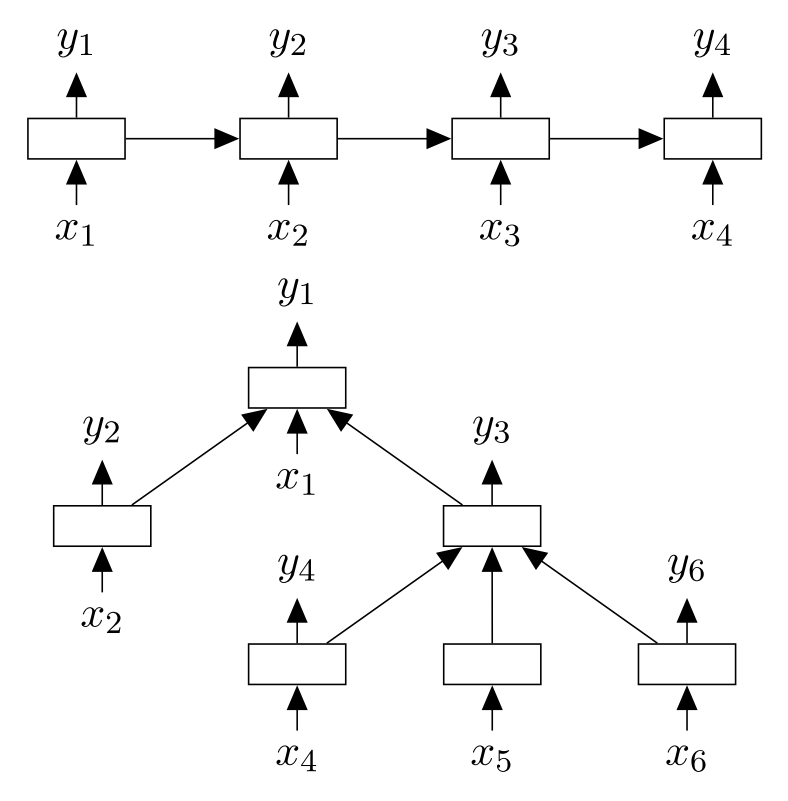
\includegraphics[width=0.7\linewidth]{img/tree-lstm.png}
    \caption{Standard LSTM (top) and tree-LSTM (bottom) (adapted from \cite{DBLP:conf/acl/TaiSM15})}
    \label{fig:tree-lstm}
\end{figure}

In contrast, \cite{DBLP:journals/corr/abs-1711-04231} kept the sequence-based LSTM intact.
However, they replaced the global attention (\cref{the-mt-att}) with their syntax-directed attention.
The proposed attention is analogous to Luong's local attention.
The only difference is how the distance between two words of the source sentence is computed.
In Chen's syntax-directed attention, the distance is the minimum number of edges to be traversed to reach one node from another in the dependency tree.
While in Luong's, it is the sequential distance.

In a simpler way, \cite{DBLP:conf/acl/LiXTZZZ17} proposed to incorporate a sequence of structural label (POS tags) to the encoder's attention by feeding these tags to an RNN.
While not actually focusing on enhancing the encoder, \cite{DBLP:conf/naacl/CohnHVYDH16} introduced structural biases to the encoder-decoder attention function.
These biases include the relative position between the target and source tokens, fertility, Markov condition and bilingual symmetry.
Using this approach, researchers enabled the decoder to attend better to hidden states of the encoder.
It was reported that the proposed approach brought consistent improvements comparing to the attentional model (\seq2seq with Bahdanau's attention).

\section{Multi-Tasking}
\label{lit-mult}

By jointly training the model to parse and translate simultaneously, it is expected that one task can be improved using the knowledge induced from the other task.
\citet{DBLP:conf/acl/EriguchiTC17} combined the translation and dependency parsing tasks by sharing the translation encoder hidden states with the buffer hidden states in a shift-reduce parsing model \cite{DBLP:conf/naacl/DyerKBS16}.

While aiming at the same goal, \citet{DBLP:conf/acl/AharoniG17a} proposed a very simple method.
Instead of modifying the model structure, they represented the target sentence as a linearized, lexicalized constituency tree.
Subsequently, a \seq2seq model was used to translate the source sentence to this linearized tree, i.e. indeed performing the two tasks.
\citet{DBLP:conf/ijcnlp/LeMYM17} made use of the same trick on, however, the dependency tree, proposing a tree-traversal algorithm to linearize the dependency tree.
Unfortunately, their algorithm was not able to traverse a non-projective tree.

The evidence presented in these papers suggests that there is improvement on the BLEU score \citep{BLEU}.
The performance in the secondary task, i.e. parsing, is however not reported.
Going toward the opposite direction, \citet{DBLP:conf/emnlp/ShiPK16} have done an in-depth analysis to further examine the usefulness of NMT model when it came to syntactic parsing. Their work pointed out which type of syntactic relations/labels were better predicted by the \seq2seq MT model.

Aiming to improve both tasks, \cite{tran2018inducing} used two different components in the encoder, one to produce the content and the other to produce the dependency matrix.
While the content is the output of the standard bidirectional LSTM as in the vanilla \seq2seq model, the dependency matrix is produced by a head word selection layer, which is modelled by self-attention (\cref{lit-trans-pos}).
Then both are fed to the decoder using a modified encoder-decoder attentional layer.
In fact, this model is enriching the decoder while still learning to do multi-tasking.

Thus far, most of the multitask models employ another neural network as the parser that is plugged into the NMT system.
Hence, this parser is able to make use of several shared layers with the NMT model.
We would argue that this commonly used setting could hardly answer our question if the translation's encoder is able to capture the source syntax.
The reason is the nature of the input to the parser, which is also the output of the shared layers.
The parser itself is a neural network or another kind of classifier that is complex enough to synthesize lower-level information for its parsing task.
That is to say the input to the parser does not need to be syntactic information.
Therefore, one cannot conclude our second research question even if the parser performs perfectly in the joint model.

In summary, the evidence presented in the literature suggests that various methods to feed syntactic information to NMT helped translation. However, little is known about whether or not NMT already captures syntactic information within the model itself, which is one of the two main questions we attempt to answer with our proposals in the following sections.

\section{The \transformer Model}
\label{lit-trans}

Before starting to discuss our main proposals in the next chapter. We would like to briefly introduce the reader to a novel NMT model that has established the state-of-the-art results in translation - the \transformer model \citep{DBLP:conf/nips/VaswaniSPUJGKP17}.
This model has three interesting features which all of our proposed methods exploit and are built upon: the self-attention mechanism, multi-head attention and the positional encoding.

\subsection{Self-Attention}
\label{lit-trans-att}

The previous studies, reviewed in \cref{lit-enc,lit-mult}, have examined mostly the \seq2seq model with RNNs (LSTMs) as the backbone, whose component is hard to exploit and modify.
The purpose of (bidirectional) LSTMs in the encoder and decoder is to learn the representation of one token using information from its neighbors.
The \transformer model eliminates the need for LSTMs in both encoder and decoder and replaces them with self-attention layers.
These self-attention layers were introduced by \cite{cheng-dong-lapata:2016:EMNLP2016}, which they called intra-attention.
They have been used in natural language inference, sentiment analysis and language modelling.
The \textit{intra-} or \textit{self-} prefixes suggest that this attention mechanism works within the input sentence, instead of between encoder and decoder as in \cref{the-mt-att}. Although the procedures to compute these two types of attention are similar, the attention layer in the \transformer has to perform an additional projection step. 

\cref{fig:self-att-layer} exhibits one typical attention layer in the \transformer, which includes the following steps:
\begin{enumerate}
    \item Project the input $x_i$ to $k_i, v_i, q_i$ using projection matrices $W^K, W^V, W^Q$, respectively.
    \item Compute the attention energy $e_{i,j}$ by a dot product of query $q_i$ and key $v_i$, divided by the dimension $d_k$ of the key.
    \item Compute the attention weight $a_{i,j}=\frac{exp(e_{i,j})}{\sum_{t}exp(e_{i,t})}$.
    \item Compute the output $o_i = \sum_{j} a_{i,j}v_j$.
\end{enumerate}

\begin{figure}[t]
    \centering
    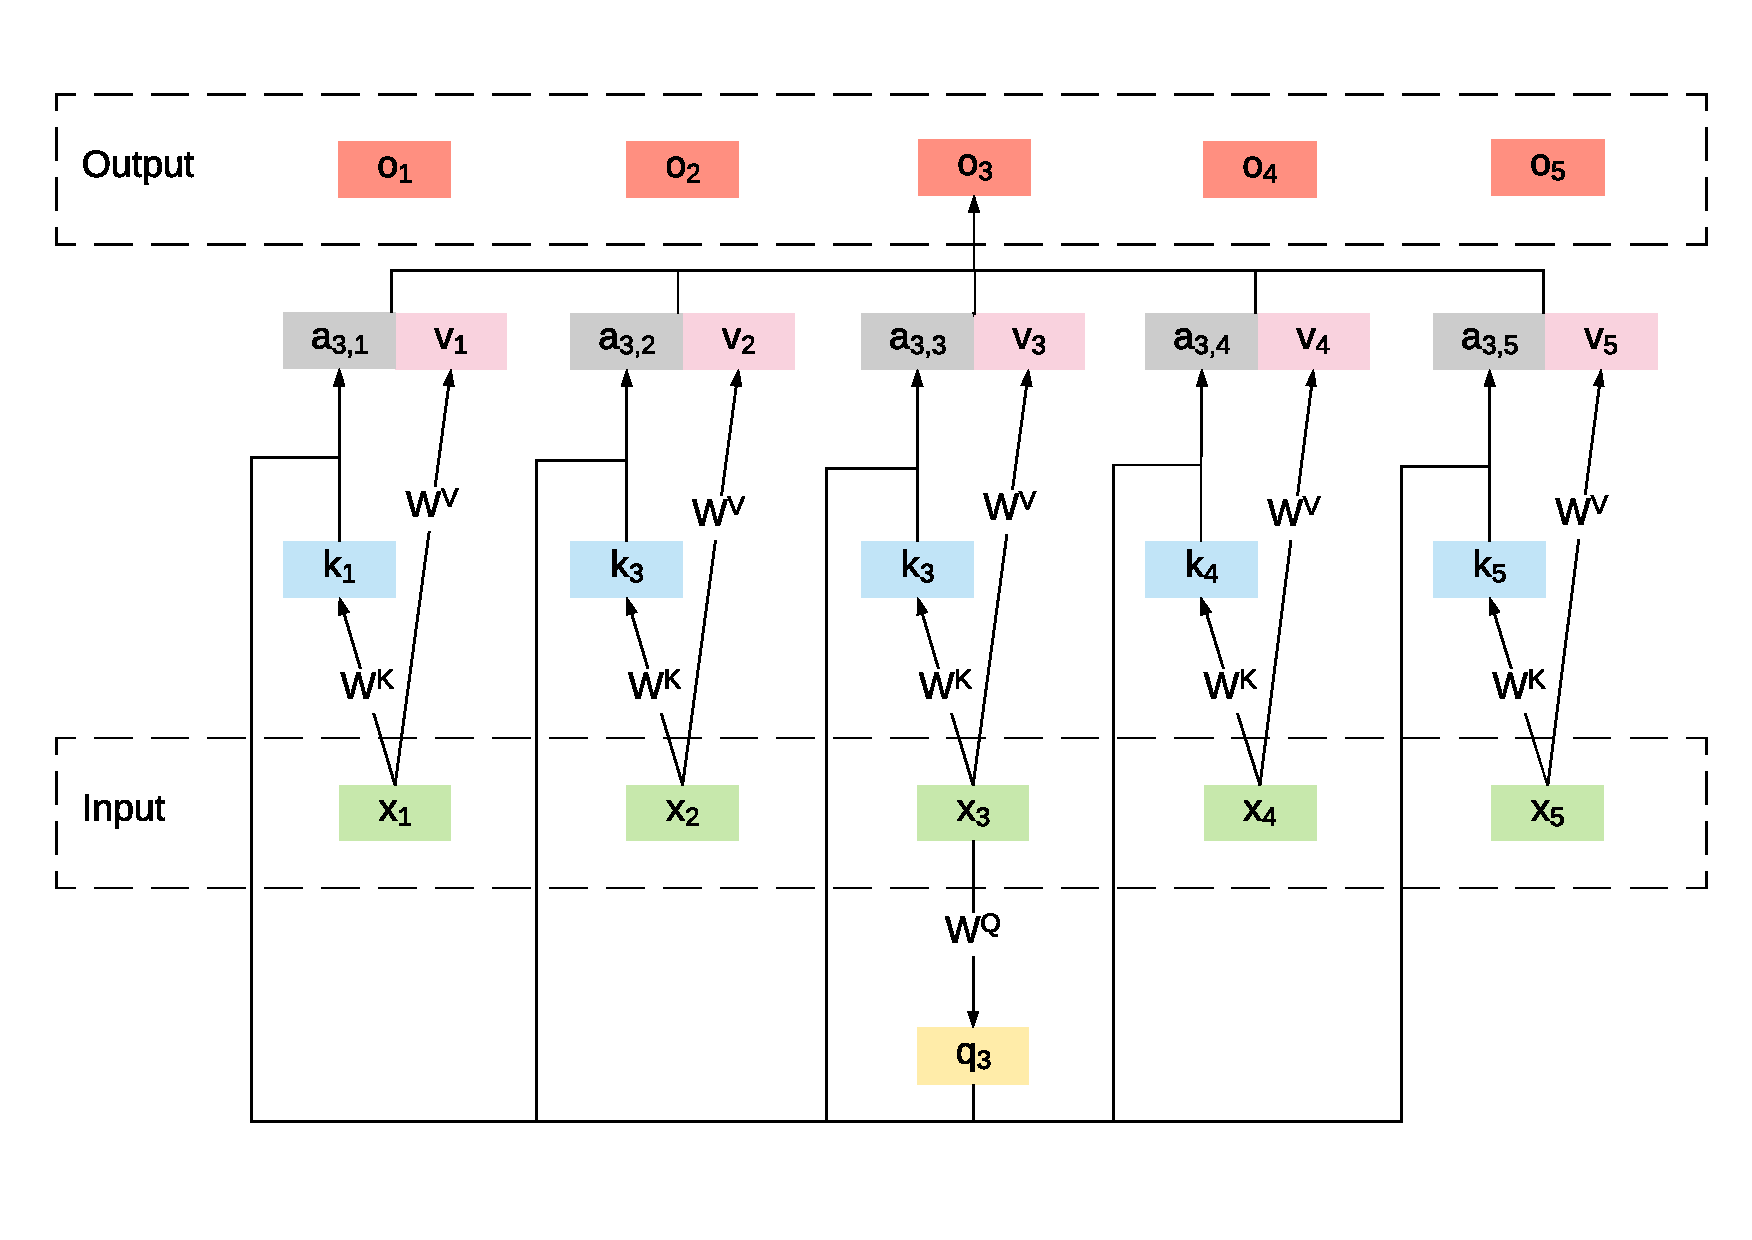
\includegraphics[width=\linewidth]{img/self-att.pdf}
    \caption{A self-attention layer in the \transformer, computing the output $o_3$.}
    \label{fig:self-att-layer}
\end{figure}

\cref{fig:self-att-sample} illustrates an example of attention weight in a self-attention layer.

\begin{figure}[t]
    \centering
    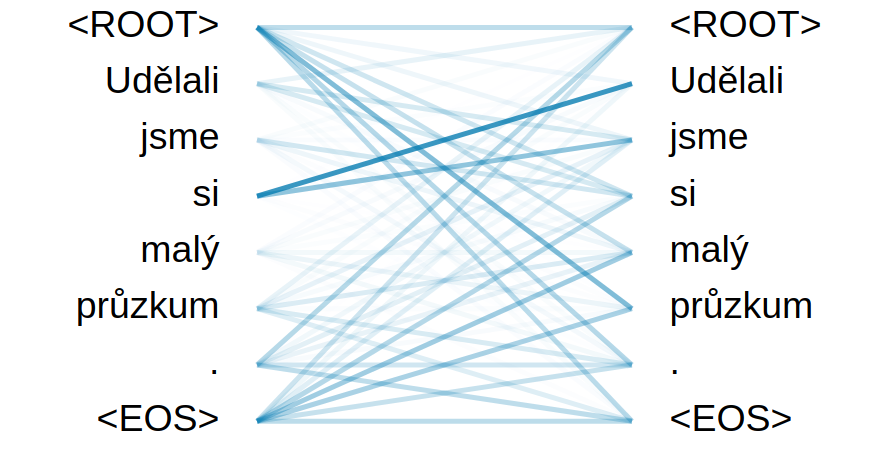
\includegraphics[width=0.6\linewidth]{img/self-att-sample.png}
    \caption{Self-attention example. The visibility of lines denotes attention weight between the layer's output (right) and layer's input (left).}
    \label{fig:self-att-sample}
\end{figure}

One significant advantage of self-attention over RNN is that the network can process in parallel. Parallelization within the layer in RNN is impossible because of the sequential nature of this structure.

\subsection{Multi-Head Attention}

The paper further refined the attention layer by concatenating several attention layers into one ``multi-head attention" layer.
In \cref{fig:multihead-attention-layer}, $h$ independent attention layers are trained in parallel.
The outputs of all are concatenated, then projected through a linear layer.

\begin{figure}[t]
    \centering
    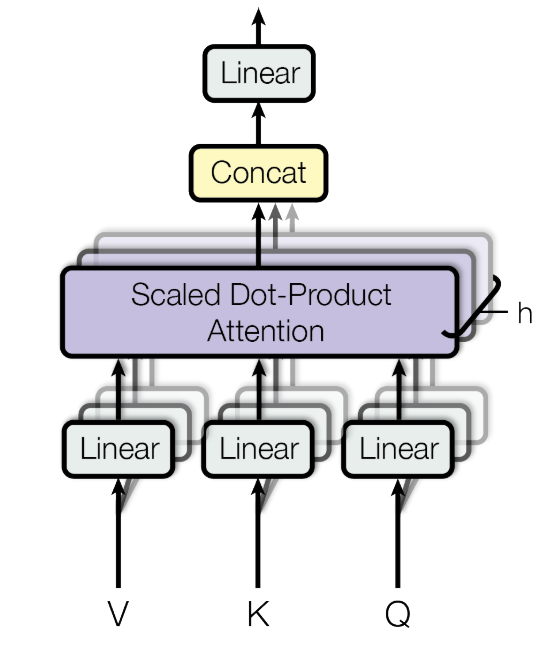
\includegraphics[width=0.5\linewidth]{img/multihead-attention.png}
    \caption{Multi-head attention layer (adapted from \cite{DBLP:conf/nips/VaswaniSPUJGKP17}).}
    \label{fig:multihead-attention-layer}
\end{figure}

This multi-head attention enhances the ability of attention mechanism in two ways:
\begin{itemize}
    \item It makes possible for the model to attend to various information at different positions. Although the attention is able to focus on several positions at one layer, multi-head attention can enable the model to attend to different patterns, and various positions in each patterns.
    For example, a noun in a sentence can attend to all related adjectives in the first attention head. In addition, it can also attend to the pronouns referring it in the second head.
    \item The multi-head attention also allows the keys, queries and values to come from multiple representation subspaces, because of different projection matrices $W^K, W^Q, W^V$ in each head.
\end{itemize}

\subsection{Positional Encoding}
\label{lit-trans-pos}

One prominent problem of replacing LSTMs with self-attention layers is that the model has no notion of token positions.
With the sequential information passing in bidirectional LSTMs, each token is aware of which tokens are before and which are after it.
The self-attention layer simply computes weights using the dot product of tokens' vectors, hence it considers the input as a bag of words.
To deal with this problem, the authors of the \transformer proposed to add a positional embedding vector to each token embedding vector before feeding it to the network.
This positional embedding vector is computed based on the token's position. Specifically, each element $i$ of the vector for the token at position $pos$ is computed by:

\[\begin{cases} \sin\left(\frac{pos}{10000^{i/d}}\right), & \mbox{if } i\mbox{ is even} \\ \cos\left(\frac{pos}{10000^{(i-1)/d}}\right), & \mbox{if } i\mbox{ is odd} \end{cases}\]

in which $d$ is the dimension of the embedding vector.

\begin{figure}
    \centering
    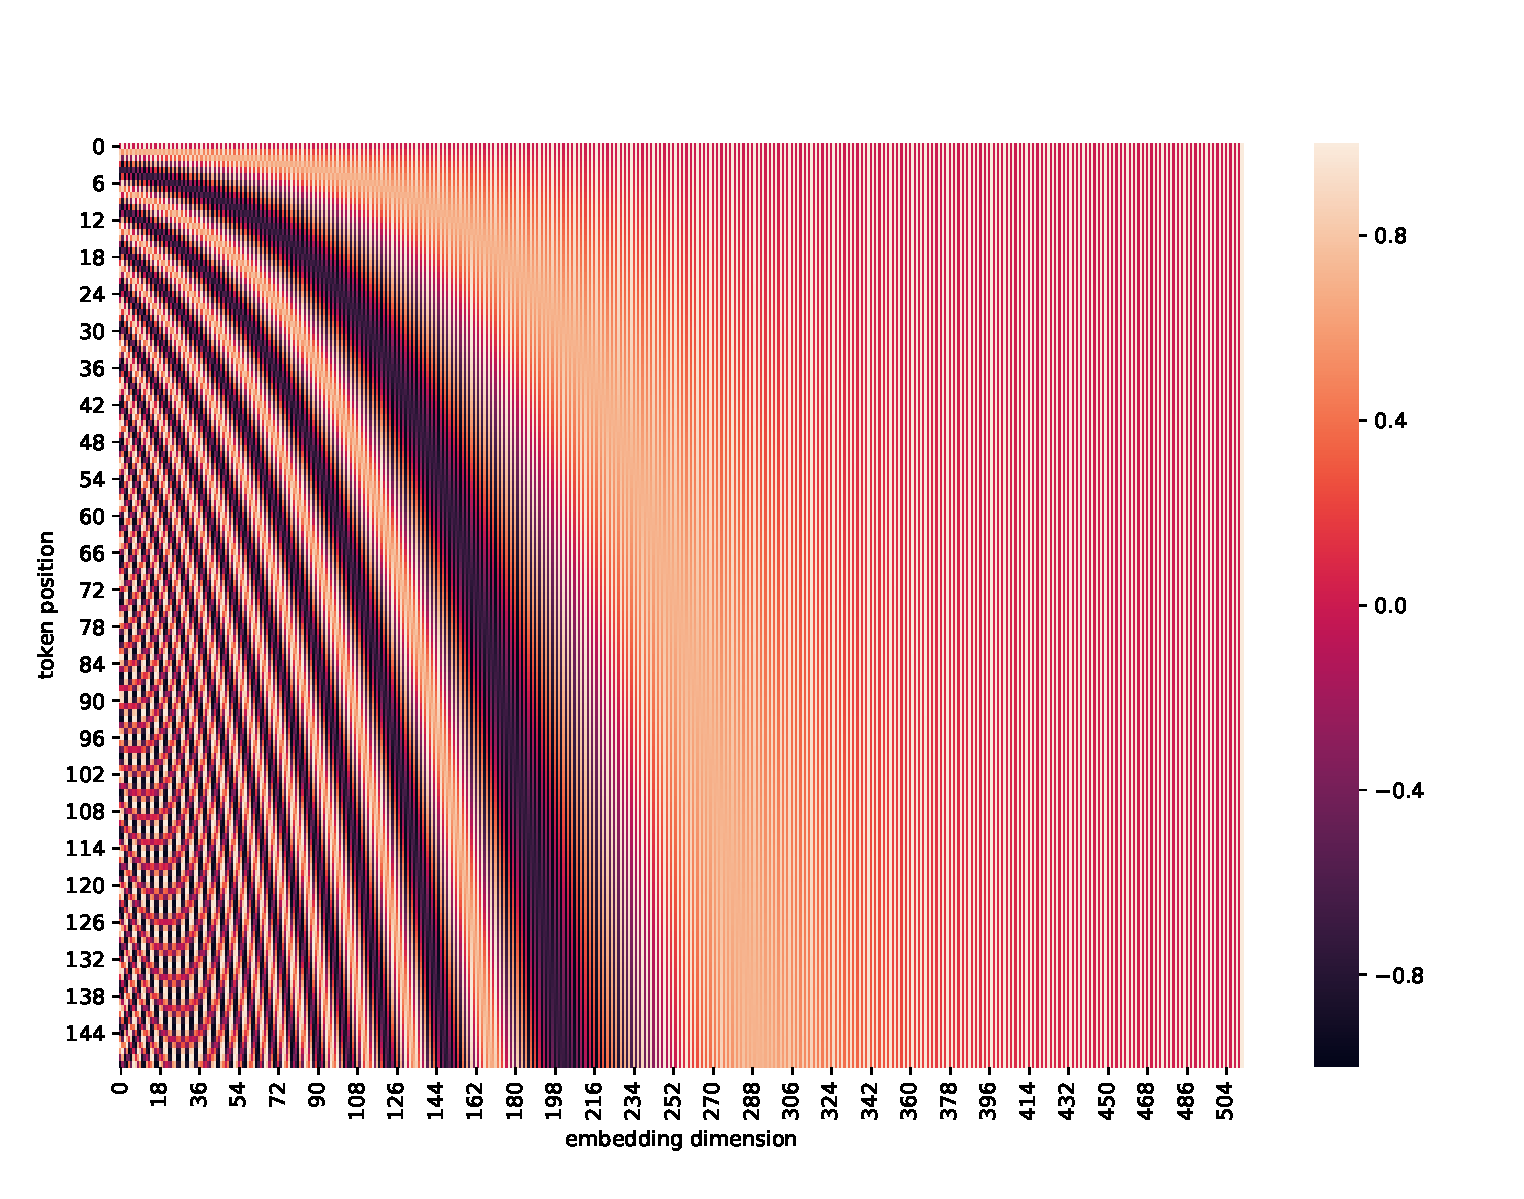
\includegraphics[width=\linewidth]{img/positional-embedding.pdf}
    \caption{Positional embeddings with sine and cosine functions, embedding size $d=512$.}
    \label{fig:positional-embedding}
\end{figure}

\cref{fig:positional-embedding} showcases the values of the generated positional embeddings (dimension of 512) for token positions ranging from 1 to 150.

The authors also experimented with the learned positional embeddings, which were trained in the same manner as word embeddings. It was reported that the two methods yielded comparable results.

\subsection{Model Architecture}
\label{lit-trans-arch}

All the features that we have discussed so far are then used to construct the \transformer model (\cref{fig:transformer}).

\begin{figure}[t]
    \centering
    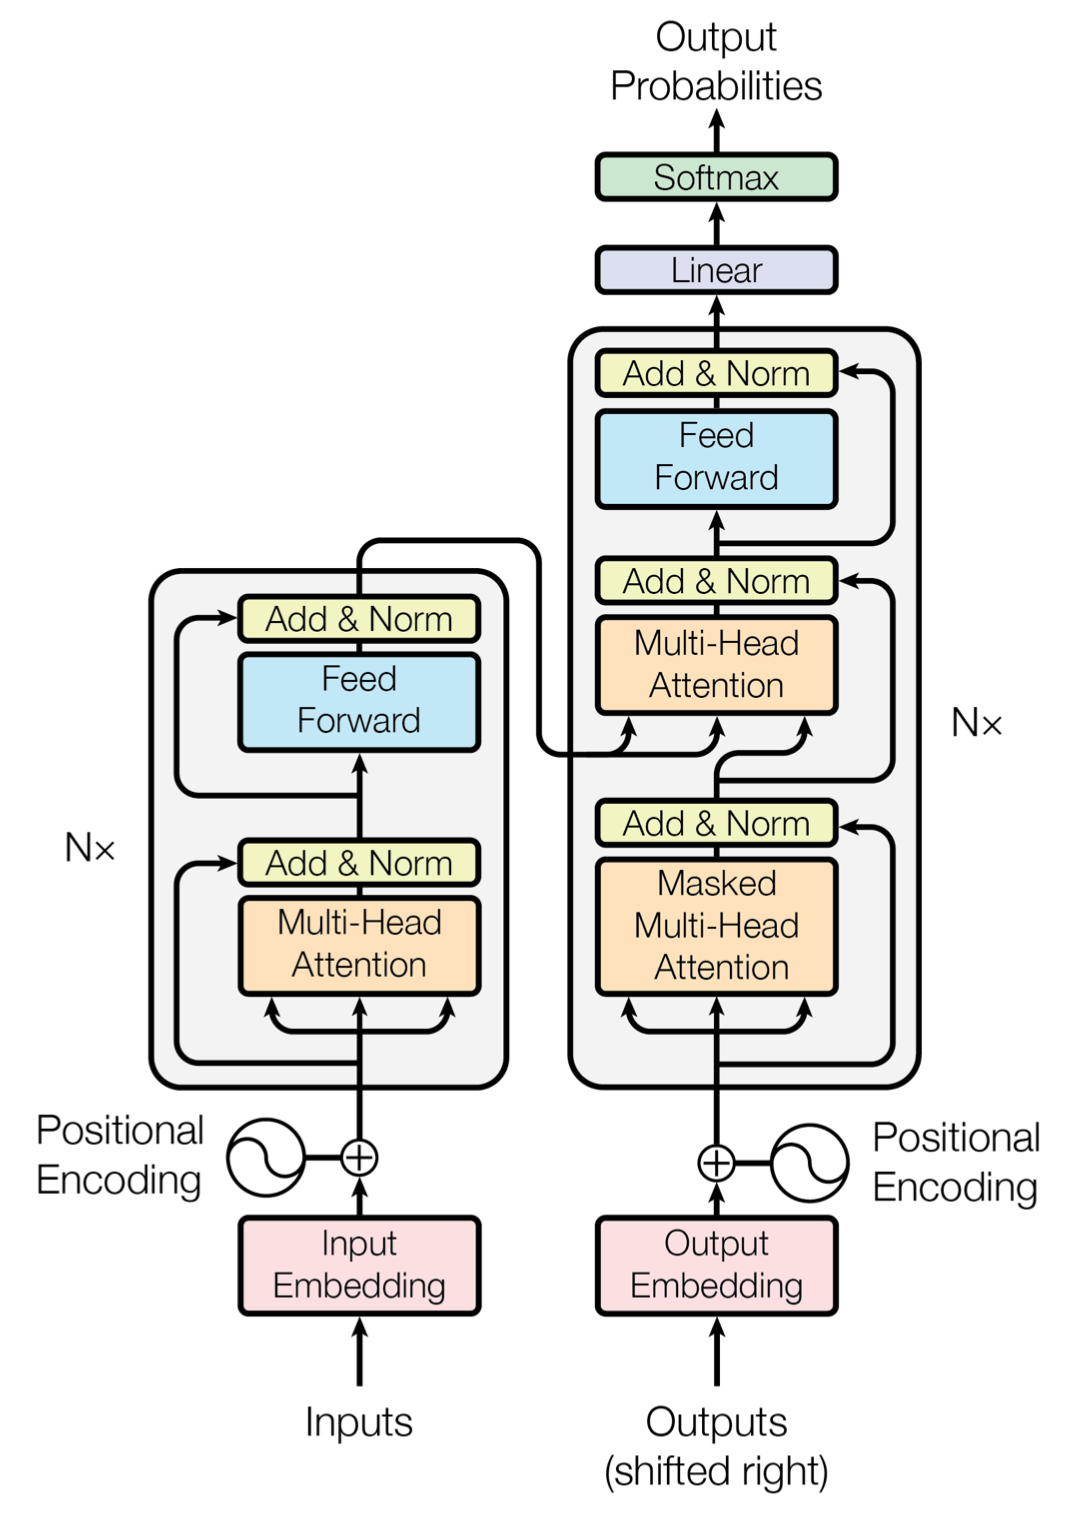
\includegraphics[width=0.9\linewidth]{img/transformer.png}
    \caption{The \transformer model (adapted from \cite{DBLP:conf/nips/VaswaniSPUJGKP17})}
    \label{fig:transformer}
\end{figure}

The model takes the input token embeddings. After being combined with the corresponding positional encoding, they are passed through the encoder, which is a stack of $N$ multi-head attention layers with projection (``feed forward") on top of each.
A similar process applies to the decoder. However, this time the multi-head attention is masked to avoid the attention layer looking into the future, i.e. it should only attend to the tokens translated up to that point.
In addition, between the masked multi-head attention and the projection layer exists another multi-head attention layer. 
This attention layer serves as the encoder-decoder attention in the \seq2seq model.
This is made possible by taking the queries from the output of the decoder's masked attention layer, while the keys and values come from the output of the encoder.
The decoder's output is then passed through another linear projection layer and finally reaches a softmax layer to produce output probabilities.

It is also important to remind the reader that there are several residual connections in \cref{fig:transformer} in which the information flow skips a multi-head attention or feed forward layer and is then recombined with the output of that layer in the ``Add \& Norm" layer.
This ``Add \& Norm" layer also performs the layer-normalization step, which is shown to be useful for the \seq2seq model.\footnote{While its counter-part - the batch-normalization performs well on the computer vision tasks with the convolutional neural network.}
